\documentclass[a4paper,11pt,twoside]{ThesisStyle}
\usepackage{etex}

\usepackage{fancyhdr}

\usepackage[left=1.4in,right=1.3in,top=1.1in,bottom=1.1in,includefoot,includehead,headheight=13.6pt]{geometry}

% Table of contents for each chapter
\usepackage[nottoc, notlof, notlot]{tocbibind}
\usepackage{minitoc}
\setcounter{minitocdepth}{2}
\mtcindent=15pt

% Glossary / list of abbreviations
\usepackage[intoc]{nomencl}
\renewcommand{\nomname}{List of Abbreviations}
\makenomenclature

%%%%%%%%%%%%%%%%%%%%%%%%%%%%%%%%%%%%%%%%%%%%%%%%%%%%%%%%%%%%%%%%%%
% ToDo Code
%%%%%%%%%%%%%%%%%%%%%%%%%%%%%%%%%%%%%%%%%%%%%%%%%%%%%%%%%%%%%%%%%%
\usepackage{xargs}
\newcommandx{\unsure}[2][1=]{\todo[linecolor=red,backgroundcolor=red!25,bordercolor=red,#1]{#2}}
\newcommandx{\change}[2][1=]{\todo[linecolor=blue,backgroundcolor=blue!25,bordercolor=blue,#1]{#2}}
\newcommandx{\info}[2][1=]{\todo[linecolor=green,backgroundcolor=green!25,bordercolor=green,#1]{#2}}
\newcommandx{\improvement}[2][1=]{\todo[linecolor=magenta,backgroundcolor=magenta!25,bordercolor=magenta,#1]{#2}}
\newcommandx{\fix}[2][1=]{\todo[linecolor=red,backgroundcolor=red!25,bordercolor=red,#1]{#2}}

%%%%%%%%%%%%%%%%%%%%%%%%%%%%%%%%%%%%%%%%%%%%%%%%%%%%%%%%%%%%%%%%%%
% PDF Code
%%%%%%%%%%%%%%%%%%%%%%%%%%%%%%%%%%%%%%%%%%%%%%%%%%%%%%%%%%%%%%%%%%

\usepackage{ifpdf}

\ifpdf
  \usepackage[pdftex]{graphicx}
  \DeclareGraphicsExtensions{.jpg}
  \usepackage[hyperindex=true]{hyperref}
\else
  \usepackage{graphicx}
  \DeclareGraphicsExtensions{.ps,.eps}
  \usepackage[dvipdfm,hyperindex=true]{hyperref}
\fi

\graphicspath{{.}{images/}}

% definitions.

\setcounter{secnumdepth}{3}
\setcounter{tocdepth}{2}

% Some useful commands and shortcut for maths:  partial derivative and stuff

\usepackage [table]{xcolor}

\newcommand{\pd}[2]{\frac{\partial #1}{\partial #2}}
\def\abs{\operatorname{abs}}
\def\argmax{\operatornamewithlimits{arg\,max}}
\def\argmin{\operatornamewithlimits{arg\,min}}
\def\diag{\operatorname{Diag}}
\newcommand{\eqRef}[1]{(\ref{#1})}

%%%%%%%%%%%%%%%%%%%%%%%%%%%%%%%%%%%%%%%%%%%%%%%%%%%%%%%%%%%%%%%%%%
% Fancy Header Style Options
%%%%%%%%%%%%%%%%%%%%%%%%%%%%%%%%%%%%%%%%%%%%%%%%%%%%%%%%%%%%%%%%%%

% Sets fancy header and footer
\pagestyle{fancy}
% Delete current footer settings
\fancyfoot{}
% Page number (boldface) in left on even
\fancyhead[LE,RO]{\bfseries\thepage}
% pages and right on odd pages
\fancyhead[RE]{\small\bfseries\nouppercase{\leftmark}}      % Chapter in the right on even pages
\fancyhead[LO]{\small\bfseries\nouppercase{\rightmark}}     % Section in the left on odd pages
\let\headruleORIG\headrule
\renewcommand{\headrule}{\color{black} \headruleORIG}
\renewcommand{\headrulewidth}{1.0pt}
\arrayrulecolor{black}

\fancypagestyle{plain}{
  \fancyhead{}
  \fancyfoot{}
  \renewcommand{\headrulewidth}{0pt}
}

% Clear Header Style on the Last Empty Odd pages
\makeatletter

\def\cleardoublepage{\clearpage\if@twoside \ifodd\c@page\else%
  \hbox{}%
  \thispagestyle{empty}%              % Empty header styles
  \newpage%
  \if@twocolumn\hbox{}\newpage\fi\fi\fi}

\makeatother

%%%%%%%%%%%%%%%%%%%%%%%%%%%%%%%%%%%%%%%%%%%%%%%%%%%%%%%%%%%%%%%%%%%%%%%%%%%%%%%
% Prints your review date and 'Draft Version' (From Josullvn, CS, CMU)
%%%%%%%%%%%%%%%%%%%%%%%%%%%%%%%%%%%%%%%%%%%%%%%%%%%%%%%%%%%%%%%%%%%%%%%%%%%%%%%
\newcommand{\reviewtimetoday}[2]{\special{!userdict begin
    /bop-hook{gsave 20 710 translate 45 rotate 0.8 setgray
      /Times-Roman findfont 12 scalefont setfont 0 0   moveto (#1) show
      0 -12 moveto (#2) show grestore}def end}}

\newenvironment{maxime}[1]
{
\vspace*{0cm}
\hfill
\begin{minipage}{0.5\textwidth}
\hrulefill $\:$ {\bf #1}\\
\it
}
{

\hrulefill
\vspace*{0.5cm}%
\end{minipage}
}

\let\minitocORIG\minitoc
\renewcommand{\minitoc}{\minitocORIG \vspace{1.5em}}

\newenvironment{bulletList}%
{ \begin{list}%
  {$\bullet$}%
  {\setlength{\labelwidth}{25pt}%
   \setlength{\leftmargin}{30pt}%
   \setlength{\itemsep}{\parsep}}}%
{ \end{list} }

\newtheorem{definition}{D?finition}
\renewcommand{\epsilon}{\varepsilon}

%%%%%%%%%%%%%%%%%%%%%%%%%%%%%%%%%%%%%%%%%%%%%%%%%%%%%%%%%%%%%%%%%%
% Centered page environment
%%%%%%%%%%%%%%%%%%%%%%%%%%%%%%%%%%%%%%%%%%%%%%%%%%%%%%%%%%%%%%%%%%

\newcommand{\Author}{Ahmad A Assaf}
\newcommand{\Subject}{Enabling Self Service Data Provisioning Through Semantic Enrichment of Data}

\newenvironment{vcenterpage}
{\newpage\vspace*{\fill}\thispagestyle{empty}\renewcommand{\headrulewidth}{0pt}}
{\vspace*{\fill}}
\usepackage{listings}
\hypersetup{
    unicode=false,                        % non-Latin characters in Acrobat?s bookmarks
    pdftoolbar=true,                      % show Acrobat?s toolbar?
    pdfmenubar=true,                      % show Acrobat?s menu?
    pdffitwindow=false,                   % window fit to page when opened
    pdfstartview={FitH},                  % fits the width of the page to the window
    pdftitle={My title},                  % title
    pdfauthor={Author},                   % author
    pdfsubject={Subject},                 % subject of the document
    pdfcreator={Author},                  % creator of the document
    pdfnewwindow=true,                    % links in new window
    colorlinks=true,                      % false: boxed links; true: colored links
    linkcolor=cyan,                       % color of internal links
    citecolor=red,                        % color of links to bibliography
    filecolor=magenta,                    % color of file links
    urlcolor=blue                         % color of external links
}

\newlength{\plarg}
\setlength{\plarg}{16cm}
\newlength{\glarg}
\setlength{\glarg}{17cm}

%%%%%%%%%%%%%%%%%%%%%%%%%%%%%%%%%%%%%%%%%%%%%%%%%%%%%%%%%%%%%%%%%%
% Listings Definitions
%%%%%%%%%%%%%%%%%%%%%%%%%%%%%%%%%%%%%%%%%%%%%%%%%%%%%%%%%%%%%%%%%%
\colorlet{punct}{red!60!black}
\definecolor{background}{gray}{0.97}
\definecolor{delim}{RGB}{20,105,176}

\lstdefinelanguage{json}{
    basicstyle=\small\ttfamily,
    showstringspaces=false,
    breaklines=true,
    frame=lines,
    captionpos=b,
    aboveskip=3mm,
    belowskip=3mm,
    backgroundcolor=\color{white},
    literate=
      {:}{{{\color{punct}{:}}}}{1}
      {,}{{{\color{punct}{,}}}}{1}
      {[}{{{\color{delim}{[}}}}{1}
      {]}{{{\color{delim}{]}}}}{1},
}

\renewcommand{\ttdefault}{pcr}
\lstdefinelanguage{owl} {
  language=xml,
  basicstyle={\footnotesize\ttfamily},
  numbers=none,
  backgroundcolor=\color{white},
  aboveskip=3mm,
  belowskip=3mm,
  showstringspaces=false,
  columns=flexible,
  keywordstyle={\bfseries\color{blue}},
  commentstyle={\color{red}\textit},
  stringstyle=\color{magenta},
  frame=lines,
  breaklines=true,
  breakatwhitespace=true,
  tabsize=4,
  morekeywords={rdf,rdfs,owl},
  moredelim=*[s][\ttfamily]{:}{:} %Newly added line
}

\listfiles

\newcommand\CyrGuillemot{%
  \def\selectguillfont{\fontencoding{OT2}\fontfamily{wncyr}\selectfont}
  \def\guillemotleft{\selectguillfont\symbol{60}}
  \def\guillemotright{\selectguillfont\symbol{62}}
}

\newcommand\PlGuillemot{%
  \def\selectguillfont{\fontencoding{OT4}\fontfamily{cmr}\selectfont}
  \def\guillemotleft{\selectguillfont\symbol{174}}
  \def\guillemotright{\selectguillfont\symbol{175}}
}

\newcommand\LaGuillemot{%
  \def\selectguillfont{\fontencoding{U}\fontfamily{lasy}%
    \fontseries{m}\fontshape{n}\selectfont}
  \def\guillemotleft{\selectguillfont\hbox{\symbol{40}%
    \kern-0.20em\symbol{40}}}
  \def\guillemotright{\selectguillfont\hbox{\symbol{41}%
    \kern-0.20em\symbol{41}}}
}

\newcommand\ECGuillemot{%
  \def\selectguillfont{\fontencoding{T1}\fontfamily{cmr}\selectfont}
  \def\guillemotleft{\selectguillfont\symbol{19}}
  \def\guillemotright{\selectguillfont\symbol{20}}
}

\newcommand\LMGuillemot{%
  \def\selectguillfont{\fontencoding{T1}\fontfamily{lmr}\selectfont}
  \def\guillemotleft{\selectguillfont\symbol{19}}
  \def\guillemotright{\selectguillfont\symbol{20}}
}

\newcommand\CyrGLeft{\CyrGuillemot\guillemotleft}
\newcommand\CyrGRight{\CyrGuillemot\guillemotright}
\newcommand\PlGLeft{\PlGuillemot\guillemotleft}
\newcommand\PlGRight{\PlGuillemot\guillemotright}
\newcommand\LaGLeft{\LaGuillemot\guillemotleft}
\newcommand\LaGRight{\LaGuillemot\guillemotright}
\newcommand\ECGLeft{\ECGuillemot\guillemotleft}
\newcommand\ECGRight{\ECGuillemot\guillemotright}
\newcommand\LMGLeft{\LMGuillemot\guillemotleft}
\newcommand\LMGRight{\LMGuillemot\guillemotright}

\newcolumntype{L}{>{\arraybackslash}m{13cm}}

\newcommand{\algorithmicrequire}{\textbf{Require:}}
\newcommand{\algorithmicensure}{\textbf{Ensure:}}

\usepackage{url}
\usepackage{psfrag}
\usepackage{array,xspace}
\usepackage[FIGTOPCAP]{subfigure}
\usepackage{epsfig,color}
\usepackage {mathpartir,amssymb,stmaryrd,mathtools}
\usepackage{alltt}
\usepackage{amsmath}
\usepackage{multirow}
\usepackage{color}
\usepackage{verbatim}
\usepackage{booktabs}
\usepackage{cases}
\usepackage{wrapfig}
\usepackage{algorithm}
\usepackage{algorithmic}
\usepackage{amssymb}
\usepackage{tabularx}
\usepackage{longtable}
\usepackage{booktabs}
\usepackage{subfigure}
\usepackage{multirow}
\usepackage{easylist}
\usepackage{setspace}
\usepackage{afterpage}
\usepackage{pdflscape}
\usepackage{caption}
\usepackage{xcolor,colortbl}
\usepackage{rotating}
\usepackage[colorinlistoftodos]{todonotes}
\usepackage{fancyhdr}
\usepackage{chngpage}

\usepackage{silence}

\WarningFilter{minitoc(hints)}{W0023}
\WarningFilter{minitoc(hints)}{W0024}
\WarningFilter{minitoc(hints)}{W0028}
\WarningFilter{minitoc(hints)}{W0030}
\WarningFilter{minitoc(hints)}{W0033}

\def\ttbraces{\let\.=\nobreak\chardef\{=`\{\chardef\}=`\}\chardef\|=`\\}

\newcommand{\TODO}[1]{\textcolor{red}{\textbf{[TODO:#1]}}}

\newenvironment{ttbox}{
 \begin{center}\vspace{-.5ex}
     \begin{tabular}{@{}|@{\,}c@{\,}|@{}}
\hline\\[-2ex]
\begin{minipage}[b]{.98\linewidth}
\begin{alltt}\ttbraces\small}
                     {\end{alltt}
     \end {minipage}\\[.3ex]
  \hline
\end{tabular}
\end{center}}

\newcommand{\symb}[1]{\makebox{\it #1}}
% shorthand for various frameworks

\def \proactive {ProActive}
\newcommand{\aspfun}{ASP${}_\text{fun}$\xspace}
\newcommand{\ttt}[1] {\texttt{#1}}


\newenvironment{myitemize}
{\begin{itemize}
\addtolength{\leftskip}{-1.5ex}
\vspace{-.1ex}}
{\end{itemize}\addtolength{\leftskip}{1.5ex}}

\newcommand\rbeta{\to_{\beta}}
\newcommand\rbetastar{{\to_{\beta}^*}}
\newcommand\parbeta{\Rightarrow_{\beta}}
\newcommand\gle{\sqsubseteq}
\newcommand\ttgle{\mbox{\( \gle \)}}
\newcommand\eps{\varepsilon}
\newcommand\eg{e.g.\ }
\newcommand\ie{i.e.\ }
\newcommand\cf{c.f.\ }
\newcommand\etal{{\it et al.} \ }
\newcommand\ttcl{pre\_cl}
\newcommand\ttsp{\mbox{\( sp \)}}
\newcommand\ttwp{\mbox{\( wp \)}}
\newcommand\ttRinv{R\mbox{\( ^{-1} \)}}
\newcommand\oim{\mbox{\(\llparenthesis\)}}
\newcommand\cim{\mbox{\(\rrparenthesis\)}}
\newcommand\imp\Rightarrow
\newcommand\ttrapp{"}

\newcommand\tthash{\mbox{\tt \#}}
\newcommand\ttcirc{\mbox{\( \circ\)}}
\newcommand\ttforall{\mbox{\( \forall \)}}
\newcommand\ttexists{\mbox{\( \exists \)}}
\newcommand\ttequiv{\mbox{\( \equiv \)}}
\newcommand\ttexistsun{\mbox{\( \exists^1 \)}}
\newcommand\ttin{\mbox{\(\in\)}}
\newcommand\ttnin{\mbox{\(\notin\)}}
\newcommand\ttTimes{\mbox{\(\times\)}}
\newcommand\ttalpha{\mbox{\( \alpha \)}}
\newcommand\ttbeta{\mbox{\( \beta \)}}
\newcommand\ttlam{\mbox{\( \lambda \)}}
\newcommand\ttsig{\mbox{\( \sigma \)}}
\newcommand\tteps{\mbox{\( \varepsilon \)}}
\newcommand\ttOmega{\mbox{\( \Omega \)}}
\newcommand\ttpi{\mbox{\( \pi \)}}
\newcommand\ttgam{\mbox{\( \gamma \)}}
\newcommand\ttneg{\mbox{\( \lnot \)}}
\newcommand\ttor{\mbox{\( \lor \)}}
\newcommand\ttwedge{\mbox{\( \land \)}}
\newcommand\ttimp{\mbox{\( \longrightarrow\)}}
\newcommand\ttImp{\mbox{\( \Longrightarrow\)}}
\newcommand\ttfun{\mbox{\( \Rightarrow\)}}
\newcommand\ttssubseteq{\mbox{\( \subseteq\)}}
\newcommand\ttrbeta{\mbox{\( \rbeta\)}}
\newcommand\ttred{\mbox{\( \to_R\)}}
\newcommand\ttuparrow{\mbox{\( \uparrow\)}}
\newcommand\ttfred{\mbox{\( \to_F\)}}
\newcommand\ttored{\mbox{\( \to_O\)}}

\newcommand\ttrbetastar{\mbox{\( \rbetastar\)}}
\newcommand\ttparbeta{\mbox{\( \parbeta\)}}
\newcommand\ttneq{\mbox{\( \neq \)}}
\newcommand\ttbigcup{\mbox{\( \bigcup \)}}
\newcommand\ttcap{\mbox{\( \cap \)}}
\newcommand\ttcup{\mbox{\( \cup \)}}
\newcommand\ttdef{\mbox{\( \equiv_{df} \)}}
\newcommand\ttsubset{\mbox{\( \subseteq \)}}
\newcommand\tttimes{\mbox{\( \times \)}}
\newcommand\ttvdash{\mbox{\( \vDash \)}}
\newcommand\ttvdashs{\mbox{\( \vdash \)}}
\newcommand\ttleq{\mbox{\( \leq \)}}
\newcommand\ttmapsto{\mbox{\( \mapsto \)}}
\newcommand\ttleftarrow{\mbox{\( \gets \)}}
\newcommand\ttleadsto{\mbox{\( \leadsto \)}}
\newcommand\ttrefone{\mbox{\( (1)\)}}
\newcommand\ttreftwo{\mbox{\( (2)\)}}
\newcommand\ttlbrack{\mbox{\(\llbracket\)}}
\newcommand\ttrbrack{\mbox{\( \rrbracket \)}}
\newcommand\ttstar{\mbox{\({}^*\)}}
\newcommand\ttmetaall{\mbox{\( \bigwedge \)}}
\newcommand\ttminusone{\mbox{\({}^{-1}\)}}
\newcommand{\oarrow}[3]{\,\relbar\Mapsfromchar\!#1,#2,#3\!\Mapstochar\to}


\newcommand\ttoarrow[3]{\mbox{\(\relbar\Mapsfromchar\)}#1,#2,#3\mbox{\(\Mapstochar\to_O\)}}

\newcommand\ttfarrow[3]{\mbox{\(\relbar\Mapsfromchar\)}#1,#2,#3\mbox{\(\Mapstochar\to_F\)}}
\newcommand\ttsubi{\mbox{\({}_{i}\)}}
\newcommand \keyword[1]{\textcolor{red}{\bf{#1}}}

\DeclareMathOperator{\futs}{futs}
\DeclareMathOperator{\Prim}{Prim}
\DeclareMathOperator{\Comp}{Comp}
\DeclareMathOperator{\Enqueue}{Enqueue}
\DeclareMathOperator{\findResult}{findRes}
\DeclareMathOperator{\dom}{dom}

\makeatletter
  \newcommand\tinyv{\@setfontsize\tinyv{7.5pt}{6.5}}
\makeatother

\makeatletter
\newcommand*{\gmshow@textheight}{\textheight}
\newdimen\gmshow@@textheight
\g@addto@macro\landscape{%
  \gmshow@@textheight=\hsize
  \renewcommand*{\gmshow@textheight}{\gmshow@@textheight}%
}
\def\Gm@vrule{%
  \vrule width 0.2pt height\gmshow@textheight depth\z@
}%
\makeatother

\makeatletter
\g@addto@macro{\UrlBreaks}{\UrlOrds}
\makeatother

\setstretch{1.1}
\setlength{\parindent}{0.2in}

\begin{document}

{

\begin{titlepage}

  \vspace{10mm}
  \noindent

	\begin{center}
	
\includegraphics[width=48mm]{util/figures/logo_ParisTech.pdf}
	\end{center}

  \vspace{5mm}


\center


\begin{bfseries}
  \noindent{\LARGE Enabling Self-Service Data Provisioning
  \vspace{6mm}
  \\Through Semantic Enrichment of Data}
  \vspace{15mm}

  \noindent{\Large Ahmad Assaf}
  \vspace{10mm}
\end{bfseries}


\noindent{A doctoral dissertation submitted to:}

\vspace{2mm}

\noindent{TELECOM ParisTech}

\vspace{2mm}

\noindent{in partial fulfillment of the requirements for the degree of:}

\vspace{2mm}

\noindent{\textbf{Doctor of Philosophy}}

\vspace{2mm}

\noindent{Specialty : \textsc{Computer Science and Multimedia}}

\vspace{2mm}



	%\noindent{Approved by the following examining committee:}


  %\vspace{2mm}

\begin{center}
\noindent \large
\begin{tabular}{llcl}
%       \textit{\textbf{Jury:}} &     & & \\\\
%      \textit{Reviewers:} & & & \\
%    \multicolumn{2}{l}{~~Prof.\  Geert-Jan \textsc{Houben}}    & - &  Delft University of Technology, Netherlands\\
%     \multicolumn{2}{l}{~~Dr.\  Catherine \textsc{Faron-Zucker}}   & - &  University of Nice Sophia Antipolis, France \\

% %  %    \textit{Advisor :}  &  \textsc{}    & - & \\
% % %     \textit{President :}&     & & \\
% \\
%       \textit{Examiners:}&    & & \\
%  \multicolumn{2}{l}{~~Prof.\ John  \textsc{Domingue}}           & - & Open University, United Kingdom   \\
% \multicolumn{2}{l}{~~Prof.\ Talel \textsc{Abdessalem}}           & - &  Telecom ParisTech, France \\
% \multicolumn{2}{l}{~~Dr.\ Tommaso \textsc{Di Noia}}           & - &   Polytechnic University of Bari, Italy \\

\textit{Supervisor:}&     & & \\
\multicolumn{2}{l}{~~Dr.\ Rapha\"el \textsc{Troncy}} & - & EURECOM, France \\
\multicolumn{2}{l}{~~Dr.\ Aline \textsc{S�nart}}     & - & SAP, France \\

\end{tabular}
\end{center}

\end{titlepage}

}

\vspace{3cm}

\tableofcontents

\let\cleardoublepage\clearpage
\chapter{Introduction}

Business Intelligence (BI) has always been about creating new insight for business by converting data into meaning that can be shared between people to drive change in the organization. One key aspect of creating meaning is to have a common shared understanding of information also known as Semantics.

Classic BI and even the newer Agile Visualization tools focus much of their selling features on attractive and unique visualizations. Preparing data for those visualizations however still remains the far most challenging task in most BI projects large and small. The ultimate goal of BI is to facilitate efficient decisions while eliminating some of the IT headache. Traditionally, BI approaches have been controlled by a centralized version of truth with a wall between IT and the business. Self-service data provisioning aims at removing this wall by providing intuitive dataset discovery, acquisition and integration techniques intuitively to the end user.

\section{Context and Motivation} \label{section:motivation}

Enterprises use a wide range of heterogeneous information systems in their business activities such as Enterprise Resource Planning (ERP), Customer Relationships Management (CRM) and Supply Chain Management (SCM) systems. An enterprise distributed IT landscape contains multiple systems using different technologies and data standards~\cite{Mihindukulasooriya:COLD:13}. In addition to this heterogeneity, the amount of information in enterprise databases and on-line data stores expands exponentially each year. Enterprise Big Data is not big in volume only, but in the associated file formats. The information is also often stored in unstructured and unknown formats.

Data integration is challenging as it requires combining data residing at different sources, and providing the user with a unified view of these data~\cite{Lenzerini:SIGMOD:02}. In large enterprises, it is a time and resource costly task. Various approaches have been introduced to solve this integration challenge. These approaches were primarily based on XML as the data representation syntax, Web Services to provide the data exchange protocols and Service-Oriented Architecture (SOA) as a holistic approach for distributed systems architecture and communication. However, it was found that these technologies are no sufficient to solve the integration problems in large enterprises~\cite{Frischmuth:ISWC:13,Frischmuth:SemWebJorunal:12}. Recently, ontology-based data integration approaches have been suggested where ontologies are used to describe the data, queries and mappings between them~\cite{Wache:IJCAI:01}. A slightly different approach is the use of the Linked Data paradigm~\cite{Bizer:IJSWIS:09} for integrating enterprise data. Enterprises like Google and Microsoft are not only using the Linked Data integration paradigm for their information systems, but are also aiming at building enterprise knowledge bases (like the Google Knowledge Graph powered in part by Freebase\footnote{\url{http://freebase.com}}) that act as a crystallization point for their structured data.

Data becomes more useful when it is open, widely available, in shareable formats and when advanced computing and analysis can yield from it. The quality and amount of structured knowledge available on the web make it now feasible for companies to mine this huge amount of public data and integrate it in their next-generation enterprise information management systems. An example of this external data is the Linked Open Data (LOD) cloud. From 12 datasets cataloged in 2007, it has grown today to nearly 1000 datasets containing more than 82 billion triples\footnote{\url{http://datahub.io/dataset?tags=lod}}~\cite{Bizer:IJSWIS:09}. Data is being published by both the public and private sectors and covers a diverse set of domains from life sciences to media or government data. The LOD cloud is potentially a gold mine for organizations and individuals who are trying to leverage external data sources in order to produce more informed business decisions~\cite{Boyd:Article:11}. This external data can be accessed through public data portals like \texttt{datahub.io} and \texttt{publicdata.eu} or private ones like \texttt{quandl.com} and \texttt{enigma.io}. Analyzing this new type of data within the context of existing enterprise data should bring them new or more accurate business insights and allow better recognition of sales and market opportunities~\cite{LaValle:MIT:11}.

\section{Use Case Scenario}\label{section:scenario}

To enable wide scale and efficient integration of data, there are some efforts needed from various sides. In this thesis, we tackle the issues and challenges from the point of views of two personae:

\begin{itemize}
	\item \textbf{Data Analyst:} A Data Analyst is an experienced professional who is able to collect and acquire data from multiple data sources, filter and clean data, interpret and analyze results and provide ongoing reports.
	\item \textbf{Data Portal Administrator:} A Data Portal Administrator monitors the overall health of a portal. He oversees the creation of users, organizations and datasets. Administrators try to ensure a certain data quality level by continuously checking for spam and manually enhancing dataset descriptions and annotations.
\end{itemize}

Throughout this thesis, we will present a use case scenario involving the two personae to illustrate the challenges and solutions that we provide.

In our scenario, \textbf{Dan} is a Data Analyst working with the Ministry of Transport in France. His favorite tool for crunching, manipulating and visualizing data is SAP Lumira\footnote{\url{http://saplumira.com/}}, a self-service data visualization tool that makes it easy to import data from multiple sources, perform visual BI analysis using intuitive dashboards, interactive maps, charts, and infographics. Dan receives a memo from his management to create a report comparing the number of car accidents that occurred in France for this year, to its counterpart in the United Kingdom (UK). In addition, he is asked to highlight accidents related to illegal consumption of alcohol in both countries.

After examining the ministry's records, Dan is able to collect the data needed to create his report for the French side. Dan also issues an official request to the Department of Transport in UK to collect the data needed. However, Dan knows that the process takes a long time and his management needs the report within days. Dan is familiar with the Open Data movement and starts his journey searching through different data portals in the UK.

\textbf{Paul} is a Data Portal Administrator for the \texttt{data.gov.uk}. He continuously oversees the processes of acquiring, preparing and publishing datasets. Paul always tries to ensure that the data published is of high quality and contains sufficient attached metadata to easily enable search and discovery. Paul often receives complaints about inaccurate or spam datasets. He manually removes and fixes errors while keeping open communication channels with the data-publishing departments.

%%%%%%%%%%%%%%%%%%%%%%%%%
%%%  Research Challenges  %%%
%%%%%%%%%%%%%%%%%%%%%%%%%

\section{Research Challenges} \label{section:challenges}

In the scenario presented above, both publishers (Data Portal Administrators) and users (Data Analysts) need pragmatic solutions that help them in their tasks. To enable that, there are some challenging research questions that have to be addressed. These challenges are organized in three main categories as the following:

\subsection{Dataset Integration and Enrichment}

\begin{itemize}
	\item The enterprise heterogeneous data sources raise tremendous challenges. They have inherently different file formats, access protocols or query languages. They possess their own data model with different ways of representing and storing the data. Data across these sources may be noisy (e.g. duplicate or inconsistent), uncertain or semantically similar but yet different. \textbf{Paul} needs powerful tools to map and organize the data in order to have a unified view for these heterogeneous and complex data structures.
	\item Attaching metadata and semantic information to instances can be tricky. An entity is usually not associated with a single generic type in the knowledge base, but rather with a set of specific types which can be relevant or not given the context. \textbf{Paul} is challenged with finding the most relevant entity type within a given context.
	\item Entities play a key role in knowledge bases in general and in the Web of Data in particular. Entities like those in DBpedia, are generally described with a lot of properties. However, it is difficult for \textbf{Dan} to assess which ones are more ``important'' than others for particular tasks such data augmentation and visualizing the key facts of an entity.
	\item Social networks are not just gathering Internet users into groups of common interests, they are also helping people follow breaking news, contribute to online debates or learn from others. They are transforming Web usage in terms of users' initial entry point, search, browsing and purchasing behavior. However, integrating information from these social networks can be tricky to \textbf{Paul} due to the vast amount of data available which makes hard to spot what is relevant in a timely manner.
\end{itemize}

\subsection{Dataset Maintenance \& Discovery}

\begin{itemize}
	\item Even though popular datasets like DBPedia\footnote{\url{http://dbpedia.org}} and Freebase are well known and widely used, there are other hidden useful datasets not being used. Indeed these datasets may be useful for specialized domains, however without proper registry of topics, it is difficult for data analysts like \textbf{Dan} to find them~\cite{Lalithsena:WI:13}.
	\item The growing amount of data requires rich metadata in order to reach its full potential. This metadata enables dataset discovery, understanding, integration and maintenance. Despite the various models and vocabularies describing datasets metadata, the ability to have an overview of the dataset by inspecting its metadata can be limited. For example, \textbf{Dan} has difficulties finding datasets with a specific geographical coverage as this information is missing from almost all of the examined datasets profiles.
	\item Users, organizations and governments are empowered to publish datasets. However, data portal administrators like \textbf{Paul} need to continuously and manually check portals to detect spam and maintain high quality data.
\end{itemize}

\subsection{Dataset Quality}

Linked Data consists of structured information supported by models, ontologies and vocabularies and contains query endpoints and links. This makes data quality assurance a challenge. Despite the fact that Linked Open Data quality is a trending and highly demanded topic, very few efforts are currently trying to standardize, track and formalize frameworks to issue scores or certificates that will help data consumers in their integration tasks. Data portal administrators like \textbf{Paul} need to have an overall view of their portals quality and want to incorporate such metrics in the existing dataset profiles. On the other hand, data analysts and users like \textbf{Dan} want to know beforehand if the dataset on hand is of a certain degree of quality to be used in their reports.

%%%%%%%%%%%%%%%%%%%%%%%%%
%%%  Thesis Contributions  %%%
%%%%%%%%%%%%%%%%%%%%%%%%%

\section{Thesis Contributions} \label{section:contribution}

In this thesis, we propose a framework to enable self-service data provisioning for internal and external data sources in the enterprise. The framework contributes to the three main challenges described above. In summary, the main contributions of this work are as follows:

\begin{adjustwidth}{-.4in}{-.4in}
	\begin{figure}[!ht]
	  \centering
	  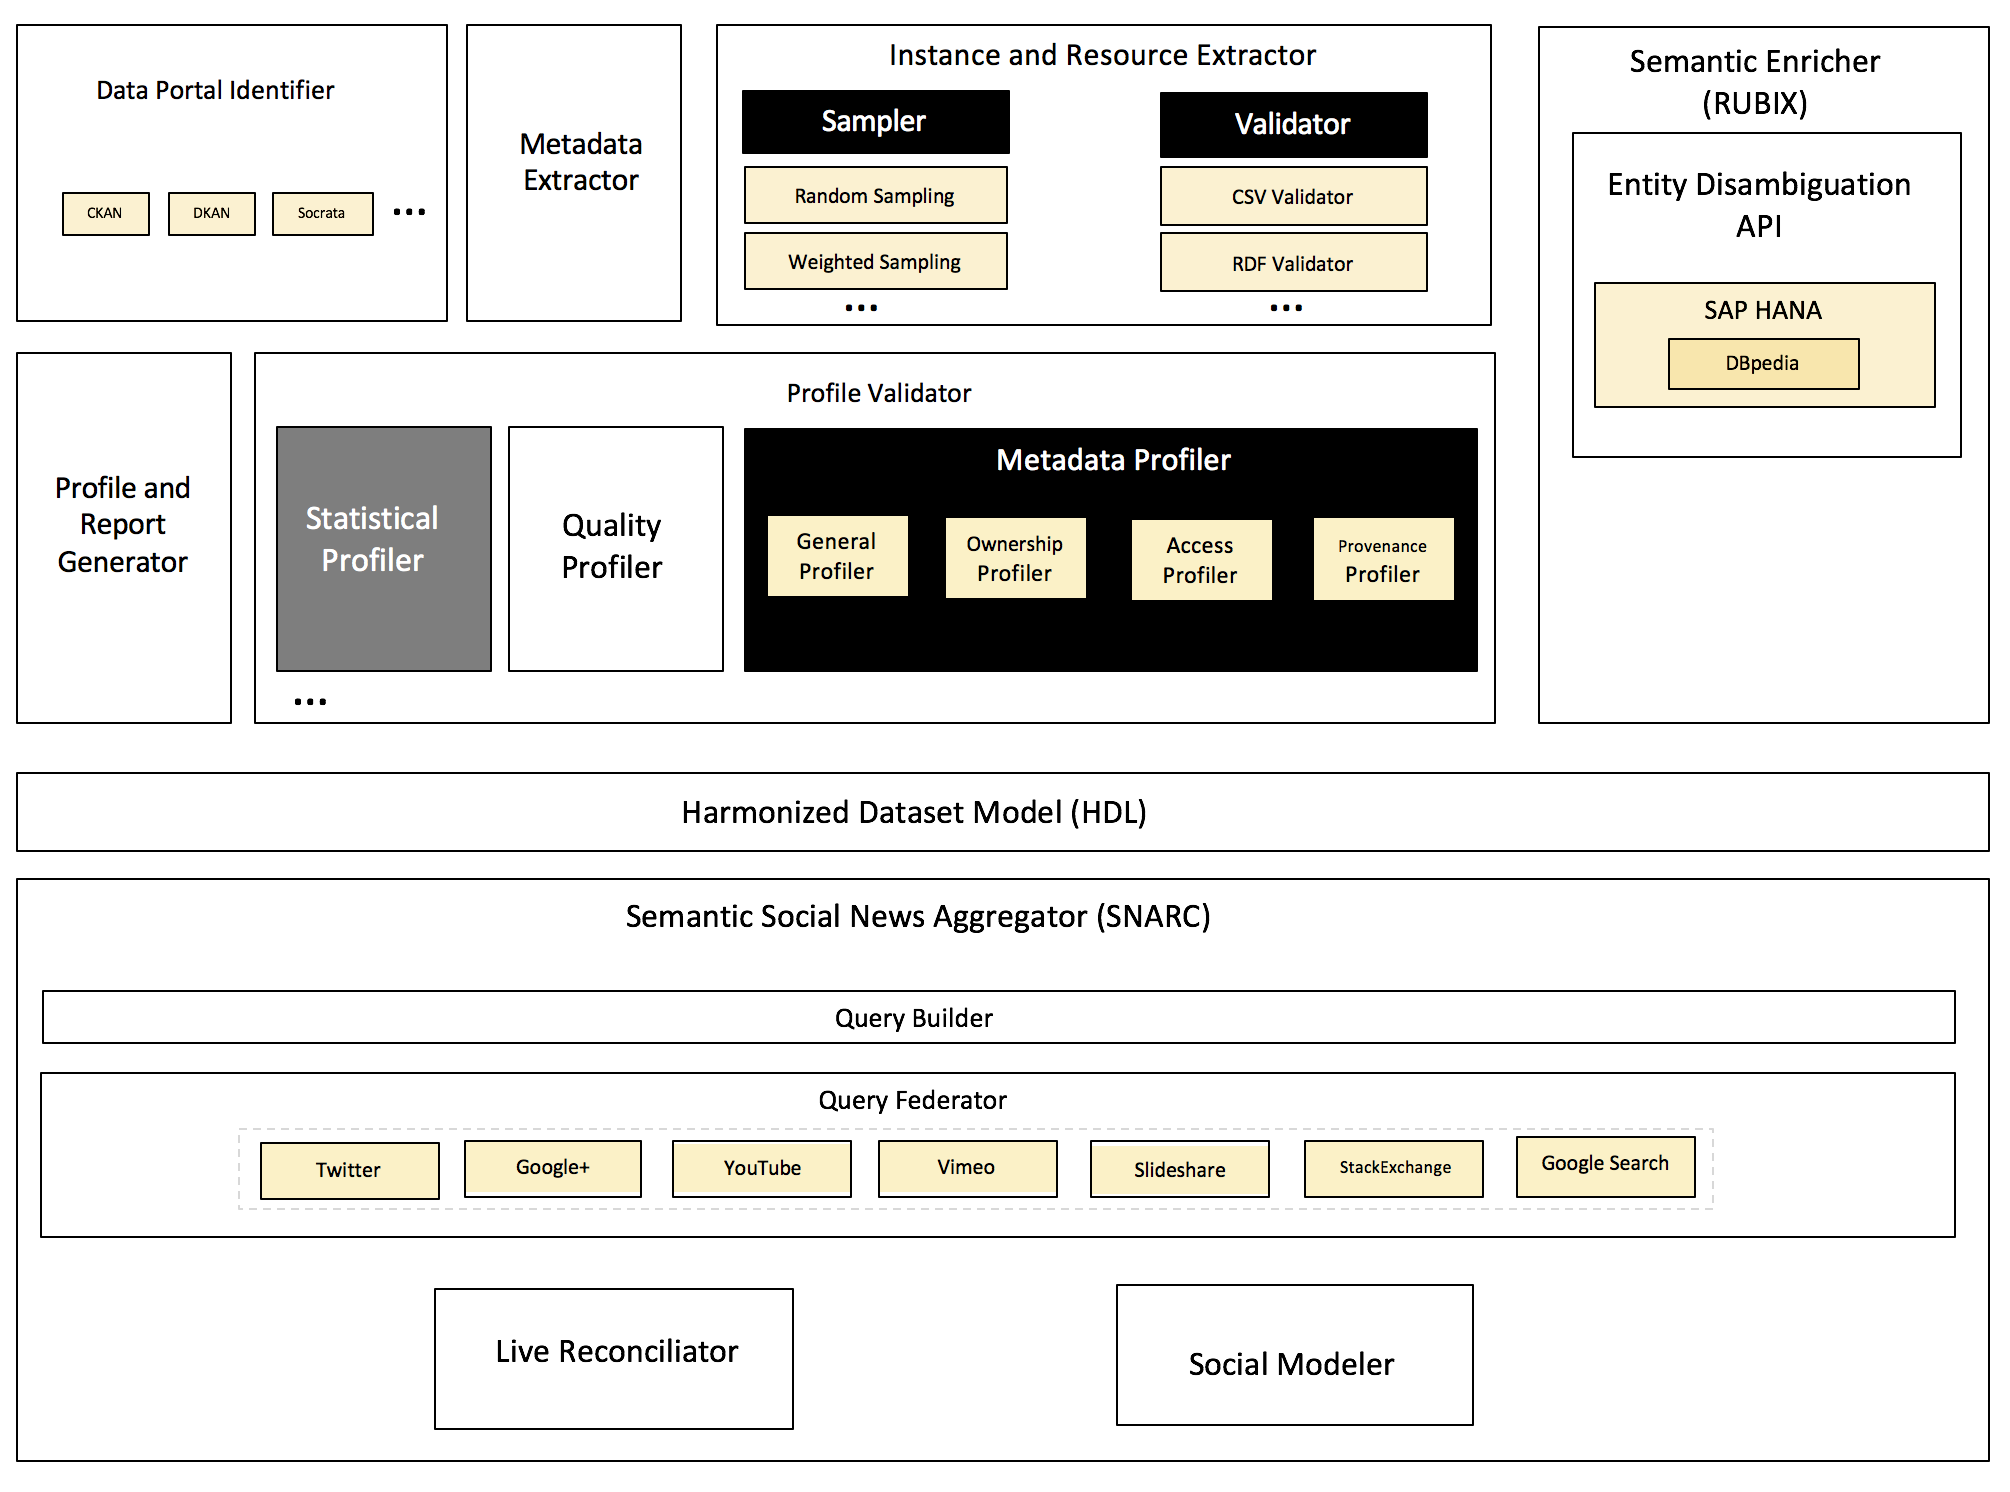
\includegraphics[scale=0.4]{figures/architecutre_diagram.png}
	  \caption{Architecture diagram for enabling self-service data provisioning}
	  \label{fig:architecutre_diagram}
	\end{figure}
\end{adjustwidth}

\subsection{Contributions on Dataset Maintenance \& Discovery}

Regarding this aspect of our research, we have achieved the following tasks:
\begin{itemize}
	\item We surveyed the landscape of various models and vocabularies that describe datasets on the web. Since establishing a common vocabulary or model is the key to communication, we identified the need for an harmonized dataset metadata model containing sufficient information so that consumers can easily understand and process datasets. First, we implemented a set of mappings between each properties of the surveyed models. This has lead to the design of HDL, a harmonized dataset model, that takes the best out of these models and extends them to ensure complete metadata coverage to enable data discovery, exploration and reuse.
	\item We have analyzed the landscape of dataset profiling tools and discovered various gaps. As a result, we proposed Roomba, a scalable automatic framework for extracting, validating, correcting and generating descriptive linked dataset profiles. Roomba applies several techniques in order to check the validity of the metadata provided and to generate descriptive and statistical information for a particular dataset or for an entire data portal.
\end{itemize}

\subsection{Contributions on Dataset Quality Control}
Concerning our contributions on Linked Data quality assessment, we have achieved the following tasks:
\begin{itemize}
	\item We proposed a linked data quality assessment framework focusing on the data's objective metrics. We have identified a total of 64 quality indicators that were mapped when suitable to four main categories (entity, dataset, links, models) corresponding to the core Linked Data publishing principles.
	\item Upon surveying the landscape of data quality tools, we noticed a lack in automatic tools to check the dataset quality metrics proposed in our framework. As a result, we extended Roomba to perform a set of data quality checks on Linked datasets. Our extension covers most of the quality indicators proposed with focus on completeness, correctness, provenance and licensing.
\end{itemize}

\subsection{Contributions on Dataset Integration and Enrichment}

Regarding this aspect of our research, we have achieved the following tasks:
\begin{itemize}
	\item We created a framework called RUBIX that enables mashing-up potentially noisy enterprise data and external data. The framework leverages reference knowledge bases to annotate data with a set of semantic concepts (metadata). One of the advantages of this metadata is to enhance the matching process of heterogeneous data sources within an enterprise.
	\item The metadata attached by RUBIX can be further used to enrich existing datasets. However, concepts are often represented with a large set of properties. To better recommend the top ``important'' properties for a concept, we reversed engineer the choices made by Google when creating knowledge graph panels and presented these choices explicitly using the Fresnel vocabulary, so that any application could read this configuration file for deciding which properties of an entity is worth to enrich.
	\item Aggregating relevant social news is not an easy task. We provide an Application Programming Interface (API) that enables semantic social news aggregation called SNARC. We designed a sample frontend application leveraging SNARC's capabilities to enable users to discover relevant social news instantly.
\end{itemize}

%%%%%%%%%%%%%%%%%%%%%%%%%
%%%  Towards A Complete Dataset Profile  %%%
%%%%%%%%%%%%%%%%%%%%%%%%%
\let\cleardoublepage\clearpage\let\cleardoublepage\clearpage
\chapter{Towards A Complete Dataset Profile}\label{chapter:1}

%%%%%%%%%%%%%%%%%%%%%%%%%
%%%  Dataset Profiles and Models  %%%
%%%%%%%%%%%%%%%%%%%%%%%%%

\section{Dataset Profiles and Models}\label{chapter:hdl}

The value of Open Data is recognized when it is used. To ensure that, publishers need to enable people to find datasets easily. Data portals are specifically designed for this purpose. They make it easy for individuals and organizations to store, publish and discover datasets.

Data portals (or data catalogs) are the entry points to discover published datasets. They are curated collections of datasets metadata that provide a set of complementary discovery and integration  services.

Data portals can be public like \texttt{Datahub.io} and \texttt{publicdata.eu} or private like \texttt{quandl.com} and \texttt{enigma.io}. Private portals harness manually curated data from various sources and expose them to users either freely or through paid plans. Similarly, in some public data portals, administrators manually review datasets information, validate, correct and attach suitable metadata information. This information is mainly in the form of predefined tags such as \textit{media, geography, life sciences} for organization and clustering purposes.

There are several Data Management Systems (DMS) that power public data portals. CKAN\footnote{\url{http://ckan.org}} is the world's leading open-source data portal platform powering web sites like DataHub, Europe's Public Data and the U.S Government's open data. Modeled on CKAN, DKAN\footnote{\url{http://nucivic.com/dkan/}} is a standalone Drupal distribution that is used in various public data portals as well. In addition to these tradition data portals, there is a set of tools that allow exposing data directly as RESTful APIs like \texttt{thedatatank.com}.

A dataset metadata model must contain sufficient information so that consumers can easily understand and process the data that is described. After analyzing the most prominent dataset models, we find out that a dataset can contain four main sections:
\begin{itemize}
  \item \textbf{Resources}: The actual raw data that can be downloaded or accessed directly via queryable endpoints. Resources can come in various formats such as JSON, XML or RDF.
  \item \textbf{Tags}: Descriptive knowledge about the dataset content and structure. This can range from simple textual representation to semantically rich controlled terms. Tags are the basis for datasets search and discovery.
  \item \textbf{Groups}: Groups act as organizational units that share common semantics. They can be seen as a cluster or a curation of datasets based on shared categories or themes.
  \item \textbf{Organizations}: Organizations are another way to arrange datasets. However, they differ from groups as they are not constructed by shared semantics or properties, but solely on the dataset's association to a specific administration party.
\end{itemize}

Upon close examination of the various data models, we grouped the metadata information into eight main types. Each section discussed above should contain one or more of these types. For example, resources have general, access, ownership and provenance information while tags have general and provenance information only. The eight information types are:
\begin{itemize}
 \item \textbf{General information}: The core information about the dataset (e.g., title, description, ID). The most common vocabulary used to describe this information is Dublin Core\footnote{\url{http://dublincore.org/documents/dcmi-terms/}}.
 \item \textbf{Access information}: Information about dataset access and usage (e.g., URL, license title and license URL). In addition to the properties in the models discussed above, there are several vocabularies designed specially to describe data access rights, e.g., Linked Data Rights\footnote{\url{http://oeg-dev.dia.fi.upm.es/licensius/static/ldr/}}, the Open Digital Rights Language (ODRL)\footnote{\url{http://www.w3.org/ns/odrl/2/}}.
 \item \textbf{Ownership information}: Authoritative information about the dataset (e.g., author, maintainer and organization). The common vocabularies used to expose ownership information are Friend-of-Friend (FOAF)\footnote{\url{http://xmlns.com/foaf/spec/}} for people and relationships, vCard~\cite{Iannella:W3C:14} for people and organizations and the Organization ontology~\cite{Reynolds:W3C:14} designed specifically to describe organizational structures.
 \item \textbf{Provenance information}: Temporal and historical information about the dataset creation and update records, in addition to versioning information (e.g., creation data, metadata update data, latest version). Provenance information coverage varies across the modeled surveyed. However, its great importance lead to the development of various special vocabularies like the Open Provenance Model\footnote{\url{http://open-biomed.sourceforge.net/opmv/}} and PROV-O~\cite{Lebo:W3C:13}. DataID~\cite{Brummer::ICSS:14} is an effort to provide semantically rich metadata with focus on providing detailed provenance, license and access information.
 \item \textbf{Geospatial information}: Information reflecting the geographical coverage of the dataset represented with coordinates or geometry polygons. There are several additional models and extensions specifically designed to express geographical information. The Infrastructure for Spatial Information in the European Community (INSPIRE) directive\footnote{\url{http://inspire.ec.europa.eu/}} aims at establishing an infrastructure for spatial information. Mappings have been made between DCAT-AP and the INSPIRE metadata. CKAN provides as well a spatial extension\footnote{\url{https://github.com/ckan/ckanext-spatial}} to add geospatial capabilities. It allows importing geospatial metadata from other resources and supports various standards (e.g., ISO 19139) and formats (e.g., GeoJSON).
 \item \textbf{Temporal information}: Information reflecting the temporal coverage of the dataset (e.g., from date to date). There has been some notable work on extending CKAN to include temporal information. \texttt{govdata.de} is an Open Data portal in Germany that extends the CKAN data model to include information like \texttt{temporal\_granularity}, \texttt{temporal\_coverage\_to} and \\\texttt{temporal\_granularity\_from}.
 \item \textbf{Statistical information}: Statistical information about the data types and patterns in datasets (e.g., properties distribution, number of entities and RDF triples). This information is particularly useful to explore a dataset as it gives detailed insights about the raw data when provided properly. VoID is the only model that provides statistical information about a dataset. VoID defines properties to express different statistical characteristics of datasets like the total number of triples, total number of entities, total number of distinct classes, etc. However, there are other vocabularies such as SCOVO~\cite{Hausenblas:ESWC:09} that can model and publish statistical data about datasets.
 \item \textbf{Quality information}: Information that indicates the quality of the dataset on the metadata and instance levels. In addition to that, a dataset should include an openness score that measures its alignment with the Linked Data publishing standards~\cite{Berners-Lee:W3C:06}. Quality information is only expressed in the POD metadata. However, \texttt{govdata.de} extends the CKAN model also to include a \texttt{ratings\_average} field. Moreover, there are various other vocabularies like daQ~\cite{Debattista:WWW:14} that can be used to express datasets quality. The RDF Review Vocabulary\footnote{\url{http://vocab.org/review/}} can also be used to express reviews and ratings about the dataset or its resources.
\end{itemize}

Since establishing a common vocabulary or model is the key to communication, we identified the need for an harmonized dataset metadata model containing sufficient information so that consumers can easily understand and process datasets. To create the mappings between the different models, we performed various steps:
\begin{itemize}
  \item Examine all the models and vocabularies specifications and documentations.
  \item Examine existing datasets using these models and vocabularies. Data Portals\footnote{\url{http://dataportals.org}} provides a comprehensive list of Open Data Portals from around the world. It was our entry point to find out portals using CKAN or DKAN as their underlying DMS. We also investigated portals known to be using specific DMS. Socrata, for example, maintains a list of Open Data portals using their software on their homepage such as \url{http://pencolorado.org} and \url{http://data.maryland.gov}.
  \item Examine the source code of some portals. This was specifically the case for Socrata as their API returns the raw data serialized as JSON rather than the dataset's metadata. As a consequence, we had to investigate the Socrata Open Data API (SODA) source code\footnote{\url{https://github.com/socrata/soda-java/tree/master/src/main/java/com/socrata/model}} and check the different classes and interfaces.
\end{itemize}

From our survey, we found that a proper integration of Open Data into businesses requires datasets to include the following information:
\begin{itemize}
	\item \textbf{Access information}: a dataset is useless if it does not contain accessible data dumps or query-able endpoints;
	\item \textbf{License information}: businesses are always concerned with the legal implications of using external content. As a result, datasets should include both machine and human readable license information that indicates permissions, copyrights and attributions;
	\item \textbf{Provenance information}: depending on the dataset license, the data might not be legally usable if there are no information describing its authoritative and versioning information. Current models under-specify these aspects limiting the usability of many datasets.
\end{itemize}

Since establishing a common vocabulary or model is the key to communication, we identified the need for a harmonized dataset metadata model containing sufficient information so that consumers can easily understand and process datasets. We have identified four main sections that should be included in the model: resources, groups, tags and organizations. Furthermore, we have classified the information to be included into eight types. Our main contribution is a set of mappings between each properties of those models. This has lead to the design of HDL, a harmonized dataset model, that takes the best out of these models to ensure complete metadata coverage to enable data discovery, exploration and reuse.

%%%%%%%%%%%%%%%%%%%%%%%%%
%%%  Dataset Profiles Generation and Validation  %%%
%%%%%%%%%%%%%%%%%%%%%%%%%
\section{Dataset Profiles Generation and Validation}\label{chapter:roomba}

The heterogeneous nature of data sources reflects directly on the data quality as they often contain inconsistent as well as misinterpreted and incomplete metadata information. Moreover, the significant variation in size, formats and freshness of the data, makes it more difficult to find useful datasets without prior knowledge. This can be clearly noticed in the LOD Cloud where few datasets such as DBPedia~\cite{Bizer:WebSemJorunal:09}, Freebase~\cite{Bollacker:SIGMOD:08} and YAGO~\cite{Suchanek::WWW:07} are favored over less popular datasets that may include domain specific knowledge more suitable for the tasks at hand. For example, for the task of building context-aware recommender systems in an academic digital library over the LOD cloud, popular datasets like the Semantic Web Dog Food\footnote{\url{http://datahub.io/dataset/semantic-web-dog-food}}, DBLP\footnote{\url{http://datahub.io/dataset/dblp}} or Yovisto\footnote{\url{http://datahub.io/dataset/yovisto}} can be favored over lesser known but more specific datasets like VIAF\footnote{\url{http://datahub.io/dataset/viaf}} which links authority files of 20 national libraries, list of subject headings for public libraries in Spain\footnote{\url{http://datahub.io/dataset/lista-encabezamientos-materia}} or the French dissertation search engine\footnote{\url{http://datahub.io/dataset/thesesfr}}.

Users explore datasets in data portals relying on the metadata information attached by either the dataset owner or the data portal administrator. This information is mainly in form of predefined tags such as \textit{media, geography, life sciences} that are used for organization and clustering purposes. However, the increasing diversity of those datasets makes it harder to classify them in a fixed number of tags that are subjectively assigned without capturing the essence and breadth of the dataset~\cite{Lalithsena:WI:13}. Furthermore, the increasing number of datasets available makes the manual review and curation of metadata unsustainable even when outsourced to communities.

Roomba is a tool we build to address the challenges of automatic validation and generation of descriptive datasets profiles. It is an extensible framework consisting of a processing pipeline that combines techniques for data portals identification, datasets crawling and a set of pluggable modules combining several profiling tasks. The framework validates the provided dataset metadata against an aggregated standard set of information. Metadata fields are automatically corrected when possible (e.g., adding a missing license URL reference). Moreover, a report describing all the issues that cannot be automatically fixed is created to be sent by email to the dataset's maintainer. There exist various statistical and topical profiling tools for both relational and Linked Data. The architecture of the framework allows to easily add them as additional profiling tasks. However, in this section, we focus on the task of dataset metadata profiling, ignoring the tasks of statistical and topical profiling. We validate our framework against a manually created set of profiles and manually check the accuracy by examining the results of running it on various CKAN-based data portals.

Roomba is built as a Command Line Interface (CLI) application using Node.js and is available on the tools Github repository\footnote{\url{https://github.com/ahmadassaf/opendata-checker/tree/master/test}}. Roomba allows data portal administrators like \textbf{Dan} to:

\begin{itemize}
  \item Fetch information about the portal's data management system
	\item Fetch all the information about datasets from a data portal
	\item Fetch all the groups information from a data portal
	\item Crawl, fetch and cache datasets (a specific dataset, datasets in a specific group, 	datasets in the whole portal)
	\item Execute aggregation report on a specific group or on the whole data portal
	\item Profile a specific dataset, a whole group or the whole data portal
\end{itemize}

Figure \ref{fig:architecutre_diagram} shows the main steps which are the following:

\begin{itemize}
	\item \textbf{Data management system identification}: The Data Portal Identifier relies on several Web scraping techniques in the identification process which includes a combination of URL inspection, meta tags inspection and Document Object Model (DOM) inspection.
	\item \textbf{Metadata extraction}: After identifying the underlying portal software, The Metadata Extractor performs iterative queries to the API in order to fetch datasets metadata and persist them in a file-based cache system. Depending on the portal software, The Metadata Extractor can issue specific extraction jobs. For example, in CKAN-based portals, The Metadata Extractor is able to crawl and extract the metadata of a specific dataset, all the datasets in a specific group (e.g., LOD cloud) or all the datasets in the portal.
	\item \textbf{Instance and resource extraction}: From the extracted metadata, the Instance and Resource Extractor is able to identify all the resources associated with that dataset. They can have various types like a SPARQL endpoint, API, file, visualization, etc. However, before extracting the resource instance(s). Considering that certain datasets contain large amounts of resources and the limited computation power of some machines on which the framework might run on, a Sampler submodule is introduced to execute various sample-based strategies as they were found to generate accurate results even with comparably small sample size of 10\%~\cite{Fetahu:ESWC:14}.
	\item \textbf{Profile validation}: The Profile Validator (component (iv)) identifies missing information and the ability to automatically correct them. Each set of metadata (general, access, ownership and provenance) is validated and corrected automatically when possible. Each profiler task has a set of metadata fields to check against. The validation process check if each field is defined and if the value assigned is valid.

	There exist many special validation steps for various fields. For example, the email addresses and URLs should be validated to ensure that the value entered is syntactically correct. In addition to that, for URLs, the Profile Validator issues an HTTP \texttt{HEAD} request in order to check if that URL is reachable. The Profile Validator also uses the information contained in a valid \texttt{content-header} response to extract, compare and correct some resources metadata values like \texttt{mimetype} and \texttt{size}.
	\item \textbf{Profile and report generation}: The validation process highlights the missing information and presents them in a human readable report. The report can be automatically sent to the dataset maintainer email if exists in the metadata. In addition to the generated report, the enhanced profiles are represented in JSON using the CKAN data model and are publicly available\footnote{\url{https://github.com/ahmadassaf/opendata-checker/tree/master/results}}.
\end{itemize}

We ran our tool on two CKAN-based data portals. The first is the Datahub targeting specifically the LOD cloud group. The current state of the LOD cloud report~\cite{Schmachtenberg:ISWC:14} indicates that the LOD cloud contains 1014 datasets. They were harvested via an LDSpider crawler~\cite{Isele:ISWC:10} seeded with 560 thousands URIs. Roomba on the other hand, fetches datasets hosted in data portals where datasets have attached relevant metadata. As a result, we relied on the information provided by the Datahub CKAN API. Examining the tags available, we found two candidate groups. The first tagged with ``lodcloud'' returned 259 datasets, while the second tagged with ``lod'' returned only 75 datasets. After manually examining the two lists, we found out the datasets grouped with the tag ``lodcloud'' are the correct ones as they contained more recent and accurate metadata. To qualify other CKAN-based portals for the experiments, we used \texttt{dataportals.org}, which contains a comprehensive list of Open Data portals from around the world. We chose the Amsterdam data portal \footnote{\url{http://data.amsterdamopendata.nl/}} as it is updated frequently and highly maintained. The portal was commissioned in 2012 by the Amsterdam Economic Board Open Data Exchange (ODE), and covers a wide range of information domains (energy, economy, education, urban development, etc.) about Amsterdam metropolitan region.

In our evaluation, we focused on two aspects: i)\textit{profiling correctness} which manually assesses the validity of the errors generated in the report, and ii)\textit{profiling completeness} which assesses if the profilers cover all the errors in the datasets metadata.

Our evaluation showed that Roomba has complete correctness and completeness for the properties examined. As a result, we ran Roomba over the LOD cloud group hosted in the Datahub. We discovered that the general state of the examined datasets needs attention as most of them lack informative access information and their resources suffer low availability. These two metrics are of high importance for enterprises looking to integrate and use external linked data. We found out that the most erroneous information for the dataset core information are ownership related since this information is missing or undefined for 41\% of the datasets. Datasets resources have the poorest metadata: 64\% of the general metadata, all the access information and 80\% of the provenance information contained missing or undefined values. We also showed that the automatic correction process can effectively enhance the quality of some information. We believe there is a need to have a community effort to manually correct missing important information like ownership information (maintainer, author, and maintainer and author emails).

\section{Objective Linked Data Quality Assessment}\label{chapter:data-quality}

We are entering an era where open is the new default. Governments, universities, organizations and even individuals are publicly publishing huge amounts of open data. This openness should be accompanied with a certain level of trust or guarantees about the quality of data. The Linked Open Data is a gold mine for those trying to leverage external data sources in order to produce more informed business decisions~\cite{Boyd:Article:11}. However, the heterogeneous nature of sources reflects directly on the data quality as these sources often contain inconsistent as well as misinterpreted and incomplete information.

Traditional data quality is a thoroughly researched field with several benchmarks and frameworks to grasp its dimensions~\cite{Kahn:ACM:02,Stvilia:ASIST:07,Wang:MIS:96}. Data quality principles typically rely on many subjective indicators that are complex to measure automatically. The quality of data in indeed realized when it is used~\cite{Juran:McGraw:99}, thus directly relating to the ability of satisfying users' continuous needs.

Web documents that are by nature unstructured and interlinked require different quality metrics and assessment techniques than traditional datasets. For example, the importance and quality of Web documents can be subjectively calculated via algorithms like Page Rank~\cite{ Page:TechReport:98}. Despite the fact that Linked Open Data quality is a trending and highly demanded topic, very few efforts are currently trying to standardize, track and formalize frameworks to issue scores or certificates that will help data consumers in their integration tasks.

Data quality assessment is the process of evaluating if a piece of data meets the consumers need in a specific use case~\cite{Bizer:WebSemantics:09}. The dimensionality of data quality makes it dependent on the task and users requirements. For example, DBpedia~\cite{Bizer:WebSemJorunal:09} and YAGO~\cite{Suchanek::WWW:07} are knowledge bases containing data extracted from structured and semi-structured sources. They are used in a variety of applications  e.g., annotation systems~\cite{Mendes:ICS:11}, exploratory search~\cite{Marie:ICS:13} and recommendation engines~\cite{DiNoia:iSemantics:12}. However, their data is not integrated into critical systems e.g., life critical (e.g., medical applications) or safety critical (e.g., aviation applications) as its data quality is found to be insufficient.

The basic idea behind Linked Data is that its usefulness increases when it is more interlinked with other datasets. Tim Berners-Lee defined four main principles for publishing data that can ensure a certain level of uniformity reflecting directly data's usability~\cite{Berners-Lee:W3C:06}:

\begin{itemize}
	\item \textbf{Make the data available on the Web}: assign URIs to identify things.
	\item \textbf{Make the data machine readable}: use HTTP URIs so that looking up these names is easy.
	\item \textbf{Use publishing standards}: when the lookup is done provide useful information using standards like RDF.
	\item \textbf{Link your data}: include links to other resources to enable users to discover more things.
\end{itemize}

\noindent
Building on these principles, we group the quality attributes into four main categories:

\begin{itemize}
	\item \textbf{Quality of the entities }: quality indicators that focus on the data at the instance level.
	\item \textbf{Quality of the dataset}: quality indicators at the dataset level.
	\item \textbf{Quality of the semantic model}: quality indicators that focus on the semantic models, vocabularies and ontologies.
	\item \textbf{Quality of the linking process}: quality indicators that focus on the inbound and outbound links between datasets.
\end{itemize}

In~\cite{Assaf:DQMST:12}, the authors identified 24 different Linked Data quality attributes. These attributes are a mix of objective and subjective measures that may not be derived automatically. In this paper, we refine these attributes into a condensed framework of 10 objective measures. Since these measures are rather abstract, we should rely on quality indicators that reflect data quality~\cite{Flemming:Thesis:10} and use them to automate calculating datasets quality.

The quality indicators are weighted. These weights give the flexibility to define multiple degrees of importance. For example, a dataset containing people can have more than one person with the same name thus it is not always true that two entities in a dataset should not have the same preferred label. As a result, the weight for that quality indicator will be set to zero and will not affect the overall quality score for the consistency measure.

Independent indicators for entity quality are mainly subjective e.g., the degree to which all the real-world objects are represented, the scope and level of details, etc. However, since entities are governed by the underlying model, we have grouped their indicators with those of the modeling quality.

Table~\ref{DQM} lists the refined measures alongside their objective quality indicators. Those indicators have been gathered by:

\begin{itemize}
	\item Transforming the objective quality indicators presented as a set of questions in~\cite{Assaf:DQMST:12} into more concrete quality indicator metrics.
	\item Surveying the landscape of data quality tools and frameworks.
	\item Examining the properties of the most prominent linked data models from the survey done in~\cite{Assaf:PROFILES:15}.
\end{itemize}


\begin{center}
{\footnotesize
\setlength\LTleft{-.5in}
\setlength\LTright{-.5in}
\begin{longtable}[h]{|c|c|c|l|}
\caption[Objective Linked Data quality framework]{Objective Linked Data quality framework} \label{DQM} \\

\hline \multicolumn{1}{|c|}{\textbf{Quality Attribute}} & \multicolumn{1}{c|}{\textbf{Quality Category}} & \multicolumn{1}{c|}{\textbf{ID}} & \multicolumn{1}{c|}{\textbf{Quality Indicator}} \\ \hline
\endfirsthead

\multicolumn{4}{c}%
{{\bfseries \tablename\ \thetable{} Objective Linked Data quality framework}} \\
\hline \multicolumn{1}{|c|}{\textbf{Quality Attribute}} &
\multicolumn{1}{c|}{\textbf{Quality Category}} & \textbf{ID} &
\multicolumn{1}{c|}{\textbf{Quality Indicator}} \\ \hline
\endhead

\multicolumn{4}{|r|}{{Continued on next page}} \\ \hline
\endfoot

\endlastfoot

\multirow{15}{*}{Completeness}
 & \multirow{5}{*}{Dataset Level} & 1 & Existence of supporting structured metadata ~\cite{Hogan:LDOW:10}\tabularnewline
\cline{3-4}
 &  & 2 & Supports multiple serializations~\cite{Zaveri:SemWebJorunal:12}\tabularnewline
\cline{3-4}
 &  & 3 & Has different data access points \tabularnewline
\cline{3-4}
 &  & 4 & Uses datasets description vocabularies \tabularnewline
\cline{3-4}
 &  & 5 & Existence of descriptions about its size \tabularnewline
 \cline{3-4}
 &  & 6 & Existence of descriptions about its structure (MIME Type, Format) \tabularnewline
 \cline{3-4}
 &  & 7 & Existence of descriptions about its organization and categorization \tabularnewline
 \cline{3-4}
 &  & 8 & Existence of information about the kind and number of used vocabularies~\cite{Zaveri:SemWebJorunal:12}\tabularnewline
\cline{2-4}
 & \multirow{1}{*}{Links Level} & 9 & Existence of dereferencable links for the dataset~\cite{Hogan:LDOW:10,Mader:TBDL:12,Gueret:ESWC:12}\tabularnewline \hline
\cline{2-4}
 & \multirow{4}{*}{Model Level} & 10 & Absence of disconnected graph clusters~\cite{Mader:TBDL:12}\tabularnewline
\cline{3-4}
 &  & 11 & Absence of omitted top concept~\cite{Hogan:LDOW:10}\tabularnewline
 \cline{3-4}
 &  & 12 & Has complete language coverage~\cite{Mader:TBDL:12}\tabularnewline
\cline{3-4}
 &  & 13 & Absence of unidirectional related concepts~\cite{Hogan:LDOW:10}\tabularnewline
 \cline{3-4}
 &  & 14 & Absence of missing labels~\cite{Mader:TBDL:12}\tabularnewline
 \cline{3-4}
 &  & 15 & Absence of missing equivalent properties~\cite{Maria:KEOD:13}\tabularnewline
 \cline{3-4}
 &  & 16 & Absence of missing inverse relationships~\cite{Maria:KEOD:13}\tabularnewline
 \cline{3-4}
 &  & 17 & Absence of missing domain or range values in properties~\cite{Maria:KEOD:13}\tabularnewline
\hline
\hline
\multirow{2}{*}{Availability} & \multirow{2}{*}{Dataset Level} & 18 & Existence of an RDF dump that can be downloaded by users~\cite{Flemming:Thesis:10}\cite{Hogan:LDOW:10}\tabularnewline
\cline{3-4}
 &  & 19 & Existence of a queryable endpoint that responds to direct queries \tabularnewline
\cline{3-4}
 &  & 20 & Existence of valid dereferencable URLs (respond to HTTP request) \tabularnewline
\hline
\hline
\multirow{3}{*}{Licensing} & \multirow{3}{*}{Dataset Level} & 21 & Existence of human and machine readable license information~\cite{Hogan:WebSemJorunal:12}\tabularnewline
\cline{3-4}
 &  & 22 & Existence of de-referenceable links to the full license information~\cite{Hogan:WebSemJorunal:12}\tabularnewline
\cline{3-4}
 &  & 23 & Specifies permissions, copyrights and attributions~\cite{Zaveri:SemWebJorunal:12}\tabularnewline
\hline
\hline
\multirow{1}{*}{Freshness} & \multirow{1}{*}{Dataset Level} & 24 & Existence of timestamps that can keep track of its modifications ~\cite{Flouris:EvoDyn:12}\tabularnewline
\hline
\hline
\multirow{11}{*}{Correctness}  & \multirow{2}{*}{Dataset Level} & 25 & Includes the correct MIME-type for the content ~\cite{Hogan:LDOW:10}\tabularnewline
\cline{3-4}
 &  & 26 & Includes the correct size for the content \tabularnewline
 \cline{3-4}
 &  & 27 & Absence of syntactic errors on the instance level~\cite{Hogan:LDOW:10}\tabularnewline
\cline{2-4}
 & \multirow{2}{*}{Links Level} & 28 & Absence of syntactic errors~\cite{Suominen:DataSemantics:13}\tabularnewline
 \cline{3-4}
 &  & 29 & Use the HTTP URI scheme (avoid using URNs or DOIs)~\cite{Mader:TBDL:12}\tabularnewline
\cline{2-4}
 & \multirow{7}{*}{Model Level} & 30 & Contains marked top concepts~\cite{Mader:TBDL:12}\tabularnewline
\cline{3-4}
 &  & 31 & Absence of broader concepts for top concepts~\cite{Mader:TBDL:12}\tabularnewline
 \cline{3-4}
 & & 32 & Absence of missing or empty labels~\cite{Acosta:ISWC:13,Mader:TBDL:12}\tabularnewline
  \cline{3-4}
 & & 33 & Absence of unprintable characters~\cite{Acosta:ISWC:13,Mader:TBDL:12} or extra white spaces in labels~\cite{Suominen:IKEM:12}\tabularnewline
\cline{3-4}
 &  & 34 & Absence of incorrect data type for typed literals~\cite{Hogan:LDOW:10,Acosta:ISWC:13} \tabularnewline
\cline{3-4}
 &  & 35 & Absence of omitted or invalid languages tags~\cite{Suominen:IKEM:12,Mader:TBDL:12}\tabularnewline
\cline{3-4}
 &  & 36 & Absence of terms without any associative or hierarchical relationships\tabularnewline
\hline
\hline
\multirow{7}{*}{Comprehensibility} & \multirow{4}{*}{Dataset Level} & 37 & Existence of at least one exemplary RDF file~\cite{Zaveri:SemWebJorunal:12}\tabularnewline
\cline{3-4}
 &  & 38 & Existence of at least one exemplary SPARQL query~\cite{Zaveri:SemWebJorunal:12}\tabularnewline
 \cline{3-4}
 &  & 39 &  Existence of general information (title, URL, description) for the dataset \tabularnewline
\cline{3-4}
 &  & 40 & Existence of a mailing list, message board or point of contact~\cite{Flemming:Thesis:10}\tabularnewline
 \cline{2-4}
 & \multirow{3}{*}{Model Level} & 41 & Absence of misuse of ontology annotations~\cite{Mader:TBDL:12,Maria:KEOD:13}\tabularnewline
  \cline{3-4}
 & & 42 & Existence of annotations for concepts~\cite{Maria:KEOD:13}\tabularnewline
 \cline{3-4}
 & & 43 & Existence of documentation for concepts~\cite{Mader:TBDL:12,Maria:KEOD:13}\tabularnewline
\hline
\hline
\multirow{3}{*}{Provenance} & \multirow{2}{*}{Dataset Level} & 44 & Existence of metadata that describes its authoritative information ~\cite{Flouris:EvoDyn:12}\tabularnewline
\cline{3-4}
 &  & 45 & Usage of a provenance vocabulary\tabularnewline
 \cline{3-4}
 &  & 46 & Usage of a versioning\tabularnewline
\hline
\hline
\multirow{10}{*}{Coherence} & \multirow{10}{*}{Model Level} & 47 & Absence of misplaced or deprecated classes or properties ~\cite{Hogan:LDOW:10}\tabularnewline
\cline{3-4}
 &  & 48 & Absence of relation and mappings clashes ~\cite{Suominen:IKEM:12}\tabularnewline
\cline{3-4}
 &  & 49 & Absence of blank nodes~\cite{Hogan:WebSemJorunal:12}\tabularnewline
\cline{3-4}
 &  & 50 & Absence of invalid inverse-functional values~\cite{Hogan:LDOW:10}\tabularnewline
\cline{3-4}
 &  & 51 & Absence of cyclic hierarchical relations~\cite{Dagobert:DL:02,Suominen:IKEM:12,Mader:TBDL:12}\tabularnewline
\cline{3-4}
 &  & 52 & Absence of undefined classes and properties usage~\cite{Hogan:LDOW:10}\tabularnewline
\cline{3-4}
 &  & 53 & Absence of solely transitive related concepts~\cite{Mader:TBDL:12}\tabularnewline
\cline{3-4}
 &  & 54 & Absence of redefinitions of existing vocabularies ~\cite{Hogan:LDOW:10}\tabularnewline
\cline{3-4}
 &  & 55 & Absence of valueless associative relations ~\cite{Mader:TBDL:12}\tabularnewline
\hline
\hline
\multirow{7}{*}{Consistency}
 & \multirow{7}{*}{Model Level}
& 56 & Consistent usage of preferred labels per language tag~\cite{Isaac:W3C:09,Mader:TBDL:12}\tabularnewline
 \cline{3-4}
 & & 57 & Consistent usage of naming criteria for concepts~\cite{Maria:KEOD:13}\tabularnewline
\cline{3-4}
 &  & 58 & Absence of overlapping labels\tabularnewline
\cline{3-4}
 &  & 59 & Absence of disjoint labels~\cite{Mader:TBDL:12}\tabularnewline
\cline{3-4}
 & & 60 & Absence of atypical use of collections, containers and reification~\cite{Hogan:LDOW:10}\tabularnewline
\cline{3-4}
 &  & 61 & Absence of wrong equivalent, symmetric or transitive relationships~\cite{Maria:KEOD:13}\tabularnewline
\cline{3-4}
 &  & 62 & Absence of membership violations for disjoint classes~\cite{Hogan:LDOW:10}\tabularnewline
\hline
\hline
\multirow{2}{*}{Security} & \multirow{2}{*}{Dataset Level} & 63 & Uses login credentials to restrict access~\cite{Zaveri:SemWebJorunal:12}\tabularnewline
\cline{3-4}
 &  & 64 & Uses SSL or SSH to provide access to their dataset~\cite{Zaveri:SemWebJorunal:12}\tabularnewline
\hline
\end{longtable}
}
\end{center}


We have extended Roomba with 7 submodules that will check various dataset quality indicators. Some indicators have to be examined against a finite set. Since Roomba runs on CKAN-based data portals, we built our quality extension to calculate the scores against the CKAN standard model.


A CKAN portal contains a set of datasets $\textbf{D} = \{D_1,...D_n\}$. We denote the set of resources $R_i = \{r_1,...,r_k\}$, groups $G_i = \{g_1,...,g_k\}$ and tags $T_i = \{t_1,...,t_k\}$ for $D_i \in \textbf{D} (i=1,...,n)$ by $  \textbf{R}=\{R_1,...,R_n\}, \textbf{G}=\{G_1,...,G_n\}$ and $\textbf{T}=\{T_1,...,t_n\}$ respectively.

Our quality framework contains a set of measures $\textbf{M} = \{M_1,...,M_n\}$. We denote the set of quality indicators $Q_i = \{q_1,...,q_k\}$ for $M_i \in \textbf{M} (i=1,...,n)$ by $\textbf{Q} = \{Q_1,...,Q_n\}$. Each quality indicator has a weight, context and a score $Q_i<weight, context, score>$. In Roomba, all the weights are equal and set to 1. However, they can be adjusted manually to rank the quality indicators. Each $Q_i$ of $M_i$ (for $i$ = 1,...$n$) is applied to one or more of the resources, tags or groups. The indicator context is defined where $\exists Q_i \in \textbf{R} \cup \textbf{G} \cup \textbf{T}$.

The quality indicator score is based on a ratio between the number of violations $\textbf{V}$ and the total number of instances where the rule applies $\textbf{T}$ multiplied by the specified weight for that indicator. In some cases, the quality indicator score is a boolean value (0 or 1). For example, checking if there is a valid metadata file (QI.1) or checking if the \texttt{license\_url} is dereferenceable (QI.22).


\begin{equation}
 Q\textrm{ weightedscore} = (V/T) * Q<weight>
\end{equation}

$Q\textrm{ weightedscore}$ is an error ratio. A quality measure score should reflect the alignment of the dataset with respect to the quality indicators. The quality measure score \textbf{M} is calculated by dividing the weighted quality indicator scores sum by the total number of instances in its context, as the following formula shows:

\begin{equation}
M =  1 - ((\sum_{i=1}^{n} Q\textrm{i weightedscore}) / \mid Qi\textrm{ context} \mid )
\end{equation}

Roomba covers 82\% of the suggested datasets objective quality indicators. Based on our experiments running Roomba on the LOD cloud, we discovered that the general state of the datasets needs attention as most of them have low completeness, provenance, licensing and comprehensibility quality scores.

%%%%%%%%%%%%%%%%%%%%%%%%%
%%%  Towards Enriched Enterprise Data  %%%
%%%%%%%%%%%%%%%%%%%%%%%%%
\let\cleardoublepage\clearpage
\chapter{Towards Enriched Enterprise Data}\label{chapter:2}

\section{Data Integration in the Enterprise}\label{chapter:rubix}
Companies have traditionally performed business analysis based on transactional data stored in legacy relational databases. The enterprise data available for decision makers was typically relationship management or enterprise resource planning data. However social media feeds, weblogs, sensor data, or data published by governments or international organizations are nowadays becoming increasingly available~\cite{Boyd:Article:11}.

The quality and amount of structured knowledge available make it now feasible for companies to mine this huge amount of public data and integrate it in their next-generation enterprise information management systems. Analyzing this new type of data within the context of existing enterprise data should bring them new or more accurate business insights and allow better recognition of sales and market opportunities~\cite{LaValle:MIT:11}.

These new distributed sources, however, raise tremendous challenges. They have inherently different file formats, access protocols or query languages. They possess their own data model with different ways of representing and storing the data. Data across these sources may be noisy (e.g. duplicate or inconsistent), uncertain or be semantically similar yet different. Integration and provision of a unified view for these heterogeneous and complex data structures therefore require powerful tools to map and organize the data.

Establishing data knowledge bases in the enterprise can facilitate the provision of data integration services~\cite{Frischmuth:SemWebJorunal:12}. In this section, we present our work in using DBpedia as an internal knowledge base. We further present a set of services that we implemented on top of DBpedia allowing entity disambiguation and enhancing schema matching. These services enable business users to semi-automatically combine potentially noisy data residing in heterogeneous silos. Semantically related data is identified and appropriate mappings are suggested to users. On user acceptance, data is aggregated and can be visualized directly or exported to Business Intelligence reporting tools. Finally, we perform a reverse engineering of the Google Knowledge graph panel to find out what are the most relevant properties for an entity. We compare these results with a survey we conducted on 152 users and show how we can represent and explicit this knowledge using the Fresnel vocabulary.

Schema matching is typically used in business to business integration, metamodel matching, as well as ETL processes. For non-IT specialists the typical way of comparing financial data from two different years or quarters, for example, would be to copy and paste the data from one Excel spreadsheet into another one, thus creating redundancies and potentially introducing copy-and-paste errors. By using schema matching techniques it is possible to support this process semi-automatically, i.e. to determine which columns are similar and propose them to the user for integration. This integration can then be done with appropriate business intelligence tools that provide visualizations.

One of the problems in performing the integration is the quality of data. The columns may contain data that is noisy or incorrect. There may also be no column headers to provide suitable information for matching. A number of approaches exploit the similarities of headers or similarities of types of column data. We proposed a new approach that exploits semantic rich typing provided by our entity disambiguation.

\subsection{Data Reconciliation}
Reconciliation enables entity disambiguation, i.e. matching cells with corresponding typed entities in case of tabular data. Google Refine already supports reconciliation with Freebase but requires confirmation from the user. For medium to large datasets, this can be very time-consuming. To reconcile data, we therefore first identify the columns that are candidates for reconciliation by skipping the columns containing numerical values or dates. We then use the disambiguation API to query for each cell of the source and target columns the list of typed entities candidates. Results are cached in order to be retrieved by our similarity algorithms.

\subsection{Matching Unnamed and Untyped Columns}
The AMC has the ability to combine the results of different matching algorithms. Its default built-in matching algorithms work on column headers and produce an overall similarity score between the compared schema elements. It has been proven that combining different algorithms greatly increases the quality of matching results~\cite{Peukert:ICDE:12}\cite{conf/wise/StracciaT05}. However, when headers are missing or ambiguous, the AMC can only exploit domain intersection and inclusion algorithms based on column data. We have therefore implemented three new similarity algorithms that leverage the rich types retrieved from Linked Data in order to enhance the matching results of unnamed or untyped columns. They are presented below.

\begin{itemize}
	\item \textbf{Cosine Similarity}: We compare the result vector of candidate types from the source column with the result vector of candidate types from the target column. The similarity $s$ between the columns pair can be calculated using the absolute value of the cosine similarity function.
	\item \textbf{Pearson Product-Moment Correlation Coefficient (PPMCC)}: The second algorithm that we implemented is PPMCC, a statistical measure of the linear independence between two variables $\left(x,y\right)$~\cite{Kowalski:RoyalStat:72}. The input for PPMC consists of two arrays that represent the values from the source and target columns, where the source column is the column with the largest set of rich types found.
	\item \textbf{Spearman's Rank Correlation Coefficient}: The last algorithm that we implemented to match unnamed and untyped columns is Spearman's rank correlation coefficient. It applies a rank transformation on the input data and computes PPMCC afterwards on the ranked data. In our experiments we used Natural Ranking with default strategies for handling ties and NaN values. The ranking algorithm is however configurable and can be enhanced by using more sophisticated measures.
\end{itemize}

\subsection{Column Labeling}

We showed in the previous section how to match unnamed and untyped columns. Column labeling is however beneficial as the results of our previous algorithms can be combined with traditional header matching techniques to improve the quality of matching.

Rich types retrieved from Freebase are independent from each other. We need to find a method that will determine normalized score for each type in the set by balancing the proportion of high scores with the lower ones using Wilson score interval for a Bernoulli parameter.

\subsection{Handling Non-String Values}

So far, we have covered several methods to identify the similarity between ``String'' values, but how about other numeral values such as dates, money, distance, etc. For this purpose, we have implemented some basic type identifier that can recognize dates, money, numerical values, numerals used as identifiers. This will help us in better match corresponding entries. Adjusting AMC's combination algorithms can be of great importance at this stage. For example, assigning weights to different matchers and tweaking the configuration can yield more accurate results.

\subsection{Important Properties for Entities}\label{Section:EKG}

Entities are generally described with a lot of properties. However, not all properties have the same importance. Some properties are considered as keys for performing instance matching tasks while other properties are generally chosen for quickly providing a summary of the key facts attached to an entity. In contrast to entities, it is difficult to assess which properties are more ``important''.

Web scraping is a technique for extracting data from Web pages. We aim at capturing the properties depicted in the Google Knowledge Panel (GKP) that are injected in search result pages~\cite{Bergman:GKG:12}. We have developed a Node.js application that queries all DBpedia concepts that have at least one instance which is \texttt{owl:sameAs} with a Freebase resource (since Freebase is the knowledge base behind the graph panel) in order to increase the probability that the search engine result page (SERP) for this resource will contain a GKP. We assume in our experiments that the properties displayed for an entity are type and context dependent (country, time, query) which can affect the results. Moreover, we filter out generic concepts by excluding those who are direct subclasses of \texttt{owl:Thing} since they will trigger ambiguous queries. We obtained a list of $352$ concepts\footnote{\url{https://github.com/ahmadassaf/KBE/blob/master/results/dbpediaConcepts.json}}.

\begin{algorithm}[ht]
\caption{Google Knowledge Panel reverse engineering algorithm} \label{algoscrapping}
\begin{algorithmic}[1]
\small
    \STATE INITIALIZE $equivalentClasses(DBpedia,Freebase) $ AS $vectorClasses$
    \STATE Upload $vectorClasses$ for querying processing
    \STATE Set $n$ AS number-of-instances-to-query
    \FOR {each $conceptType \in vectorClasses$}
	\STATE SELECT $n$ instances
	\STATE $listInstances \leftarrow$ SELECT-SPARQL($conceptType$, $n$)
		\FOR {each $instance \in listInstances$}
			\STATE CALL http://www.google.com/search?q=$instance$
			\IF {$knowledgePanel$ exists}
				\STATE SCRAP GOOGLE KNOWLEDGE PANEL
			\ELSE
				\STATE CALL http://www.google.com/search?q=$instance + conceptType$
 				\STATE SCRAP GOOGLE KNOWLEDGE PANEL
			\ENDIF
			\STATE $gkpProperties \leftarrow$ GetData(DOM, EXIST(GKP))

		\ENDFOR
	\STATE COMPUTE occurrences for each $prop \in gkpProperties$
    \ENDFOR
    \STATE $gkpProperties$
\end{algorithmic}
\end{algorithm}


Fresnel\footnote{\url{http://www.w3.org/2005/04/fresnel-info/}} is a presentation vocabulary for displaying RDF data. It specifies \textit{what} information contained in an RDF graph should be presented with the core concept \texttt{fresnel:Lens}~\cite{Pietriga:ISWC:06}.PROV-O\footnote{\url{http://www.w3.org/TR/prov-o/}} is a vocabulary to describe semantically rich metadata with focus on providing detailed provenance, license and access information.  We use those two vocabularies to explicitly represent what properties should be depicted when displaying an entity\footnote{\url{https://github.com/ahmadassaf/KBE/blob/master/results/results.n3}}. This dataset can now be re-used as a configuration for any consuming application for a snippet of the generated Fresnel file).


\section{Semantic Social News Aggregation}\label{chapter:snarc}

With the rapid advances of the Internet, social media become more and more intertwined with our daily lives. The ubiquitous nature of Web-enabled devices, especially mobile phones, enables users to participate and interact in many different forms like photo and video sharing platforms, forums, newsgroups, blogs, micro-blogs, bookmarking services, and location-based services. Social networks are not just gathering Internet users into groups of common interests, they are also helping people follow breaking news, contribute to online debates or learn from others. They are transforming Web usage in terms of users' initial entry point, search, browsing and purchasing behavior~\cite{Bakshy:WWW:12}.

A common scenario that often happens while reading an interesting article, coming across a nice video or participating in a discussion in a forum is the growing interest to check related material around the information read. To do so, users might go to Twitter, Google+ or YouTube. They can try several times with several keywords to obtain the desired results. In the end, they might end up with several browser tabs opened and get distracted by the information overload from all these resources. The same happens in companies when business users are interested in information provided by corporate web applications like enterprise communities. In this section, we present SNARC, a semantic social news aggregator that leverages live rich data that social networks provide to build an interactive rich experience on both the Internet and Intranets. The service retrieves news related to the current page from popular platforms like Twitter, Google+, YouTube, Vimeo, Slideshare, StackExchange and the Web. As a possible front-end implementation, we have created a Google Chrome extension which enriches the user experience by augmenting related contextual information to entities on the page itself, as well as displaying related social news on a floating sidebar.

The back-end of SNARC consists of three major components: a document handler that creates a ``Semantic Model'' representing any web resource, a query layer that is responsible for disseminating queries to the supported social services and a data parser which processes the search results, wraps them in a common social model and generates the desired output.

%%%%%%%%%%%%%%%%%%%%%%%%%
%%%  perspectives  %%%
%%%%%%%%%%%%%%%%%%%%%%%%%

\chapter{Achievements}

This thesis thoroughly describes the different steps aiming at realizing the vision of enabling self service data provisioning in the enterprise. The work presented is beneficial to both our personae introduced. The contributions made are: \\

\section{Contributions for Data Portals Administrators}

Our data portal administrator \textbf{Paul} is always looking to expand his portals in terms of the number of datasets hosted, without compromising in their portal's data quality. In Section~\ref{chapter:hdl}, we surveyed the landscape of various models and vocabularies that described datasets on the web. We found a shortcoming when it comes to having a complete descriptive dataset model taking into account access, license and provenance information. As a result, we proposed a Harmonized Dataset Model (HDL) that \textbf{Paul} will use as a basis to extend and present the datasets he controls. \textbf{Paul} now also knows what are the major dataset models out there, and what kind of metadata data owners need to fully represent their dataset. The mappings proposed will allow him to easily integrate data from various data management systems into his own.

In Section~\ref{chapter:roomba}, we proposed Roomba, an automatic dataset profiles generation and validation tool that can be easily extended to perform various profiling tasks. Out of the box, \textbf{Paul} can use Roomba to automatically fix datasets metadata issues, and notify the datasets owners of the other issues to be manually fixed.

In Section~\ref{chapter:data-quality}, we proposed a comprehensive objective quality framework applied to the Linked Open Data. Moreover, after surveying the landscape of existing data quality tools, we identified several gaps and the need for a comprehensive evaluation and assessment framework and specifically for measuring quality on the dataset level. As a result, we presented an extension of Roomba that covers 82\% of the suggested datasets objective quality indicators. \textbf{Paul} will be able now to identify spam and low quality datasets. In addition to that, data available in his portal will now have rich semantic information attached to it. For example, temporal and spatial information extracted will be assigned into the corresponding fields in HDL. As an exemplary result, various datasets will be easily identifiable to cover various parts of the UK.

\section{Contributions for Data Analysts}

Our data analyst \textbf{Dan} believes that ``more data beats better algorithms'' and is always hunting for high quality data to produce accurate reports to the management team. By examining the rich datasets metadata presented in HDL he will be able to make fast decisions whether the dataset examined is suitable or not. He will also have vital information about the licensing and limitations for using this data internally. He will also have assurances on the dataset quality, which will help choose the best candidates out of ranked list.

\textbf{Dan} will be able to have direct access to rich and high-quality dataset descriptions generated by Roomba. Moreover, the topical profilers in Roomba will be able to identify occurrences of alcohol related terms like ``wine'' in various datasets. Query expansion methods can be used to relate alcohol to wine allowing him to find the datasets he wants.

In Section~\ref{chapter:rubix}, we presented an entity disambiguation API built on top of SAP HANA. This API is used in RUBIX, a framework we proposed to enable mashup of potentially noisy enterprise and external data.
\textbf{Dan} now has access to various datasets that he found matching his query to the portal administered by \textbf{Paul}. He will be also able to use the schema matching services to find and merge those datasets in his reports.

Having imported those dataset into Lumira, he will be also able to use the internal knowledge base to apply various semantic enrichments on this data.

In Section~\ref{chapter:snarc}, we proposed SNARC, a semantic social news aggregation service that allows the user to explore relevant news from internal or external sources. \textbf{Dan} is also a modern person, who is always trying to fresh information and believes in the wisdom of the crowd. Having SNARC services integrated with Lumira, he is also able to see a feed of relevant social media items that can be of interest to him. He actually follows a link in some tweet that he saw and was able to find relevant pieces of pointers that he would like to investigate further.

In summary, the contributions above pave the way to build a set of smart services to enable analysts easily find relevant pieces of information and administrators fight spam and be able to maintain high quality data portals. The work presented in this thesis goes beyond the fact that attaching metadata to datasets is vital, but propose a set of services that can automatically achieve that in seamless manner.

\section{Perspectives}

This thesis could be extended in the following directions:

\subsection{Data Profile Representation}
The proposed Harmonized Dataset Model (HDL) is currently available as a hierarchical JSON file. An enhancement would be to refine HDL and present it as a fully fledged OWL ontology. In addition, HDL can be extended to propose also a set of enumerations as values to ensure a unified fine-grained representation of a dataset. Moreover, while we presented the mappings between various models in a table structure, presenting those mappings in a machine readable format will allow various tools like Roomba to use it.

\subsection{Automatic Dataset Profiling}
It has been noticed that the issues surrounding metadata quality affect directly dataset search as data portals rely on such information to power their search index. There are various extensions to our tool Roomba that can help in automatically building and enhancing dataset profiles. An example of these extension would be the integration of statistical and topical profilers allowing the generation of full comprehensive profiles. We would also like to extend Roomba to be able to run over other data portal types like DKAN or Socrata. This extension can be done by leveraging the data models mappings we proposed. In addition to all that, a possible enhancement will be ability to correct the rest of the metadata either automatically or through intuitive manually-driven interfaces.

\subsection{Objective Linked Data Quality}
Ensuring data quality in Linked Open Data is a complex process as it consists of structured information supported by models, ontologies and vocabularies and contains queryable endpoints and links. In this thesis, we managed to narrow down the set of quality issues surrounding Linked Data to those who can be objectively measured and assessed by automatic tools. Our proposed tool covers 85\% of the quality indicators proposed. A possible extension would be to integrate tools assessing models quality in addition to syntactic checkers with Roomba. This will provide a complete coverage of the proposed quality indicators. Moreover, there are currently no weights assigned to the quality indicators. A valid contribution would be to suggest weights to those indicators which will result in a more objective quality calculation process.

\subsection{Enterprise Data Integration}
A vital component to Data Integration in the enterprise is the existence of enterprise knowledge bases. Integrating additional linked open data sources of semantic types such as YAGO and evaluate our matching results against instance-based ontology alignment benchmarks such as OAEI\footnote{http://oaei.ontologymatching.org/2011/instance/index.html} or ISLab\footnote{http://islab.dico.unimi.it/iimb/} are possible future directions. Moreover, our work can be generalized to data classification. The same way the AMC helps identifying the best matches for two datasets, we plan to use it for identifying the best statistical classifiers for a sole dataset, based on normalized scores.

%%%%%%%%%%%%%%%%%%%%%%%%%
%%%  Bibliography %%%
%%%%%%%%%%%%%%%%%%%%%%%%%
\bibliographystyle{plain}
\bibliography{../../Util/Bibliography/bibliography}

\vspace{-15ex}
\end{document}
